\section{Performance Evaluation and Implementation Issues} \label{sec: Implementation}

In this section, we present selected simulation results for our proposed method, in two-layer and three-layer network settings. Further, we introduce some acceleration techniques that can speed up the algorithm and reduce computing time. 

\subsection{\normalsize Simulation Results}
For the 2-layer network, as mentioned in Section \ref{sec:set-up}, since the main target of our proposed algorithm is to provide estimates for $B^*$ and $\Theta_\epsilon^*$ (since $\Theta_X$ can be estimated separately), we only present evaluation results for $B^*$ and $\Theta_\epsilon^*$ estimates. Similarly, for the three-layer network, we only present evaluation results involving Layer 3, using the notation in Section \ref{sec:identifiability}, that is, $B^*_{XZ},B^*_{YZ}$ and $\Theta^*_{\epsilon,Z}$ estimates, which is sufficient to show how our proposed algorithm works in the presence of a 
``super" - layer, taking  advantage of the separability of the log-likelihood. 

\textbf{\textit{2-layered Network.}} To compare the proposed method with the most recent methodology that also provides estimates for the regression parameters and the precision matrix (CAPME, \cite{cai2012covariate}), we use the exact same model settings that have been used in that paper. Specifically, we consider the following two models: 
\begin{itemize}
\item Model A: Each entry in $B^*$ is nonzero with probability $5/p_1$, and off-diagonal entries for $\Theta_\epsilon^*$ are nonzero with probability $5/p_2$. 
\item Model B: Each entry in $B^*$ is nonzero with probability $30/p_1$, and off-diagonal entries for $\Theta_\epsilon^*$ are nonzero with probability $5/p_2$. 
\end{itemize}
As in \citet{cai2012covariate}, for both models, nonzero entries of $B^*$ and $\Theta_\epsilon^*$ are generated from $\mathsf{Unif}\left[(-1,-0.5)\cup(0.5,1)\right]$, and diagonals of $\Theta_\epsilon^*$ are set identical such that the condition number of $\Theta_\epsilon^*$ is $p_2$. 
\begin{table}[H]
\centering
\caption{Model Dimensions for Model A and B}
\begin{tabular}{cc}
\hline
    	& $(p_1,p_2,n)$ \\ \hline
Model A	 & $p_1=30, p_2=60, n=100$ \\
																		& $p_1=60, p_2=30, n=100$ \\
																		& $p_1=200, p_2=200, n=150$ \\														& $p_1=300, p_2=300, n=150$ \\ 
\hline
Model B& $p_1=200,p_2=200,n=100$ \\
																		& $p_1= 200, p_2=200, n=200$ \\
\hline
\end{tabular}
\end{table}

To evaluate the selection performance of the algorithm, we use sensitivity (SEN), specificity (SPE) and Mathews Correlation Coefficient (MCC) as criteria:
\begin{equation*}
\textrm{SEN} = \frac{\textrm{TN}}{\textrm{TN}+\textrm{FP}},\quad \textrm{SPE} = \frac{\textrm{TP}}{\textrm{TP}+\textrm{FN}}, \quad \textrm{MCC} = \frac{\textrm{TP}\times\textrm{TN}-\textrm{FP}\times \textrm{FN}}{\sqrt{(\textrm{TP}+\textrm{FP})(\textrm{TP}+\textrm{FN})(\textrm{TN}+\textrm{FP})(\textrm{TN}+\textrm{FN})}}.
\end{equation*}
Further, to evaluate the accuracy of the magnitude of the estimates, we use the relative error in Frobenius norm:
\begin{equation*}
\textrm{rel-Fnorm} = \frac{\|\widetilde{B}-B^*\|_\textrm{F}}{\|B^*\|_\textrm{F}}\quad \text{or}\quad \frac{\|\widetilde{\Theta}_\epsilon-\Theta_\epsilon^*\|_\textrm{F}}{\|\Theta_\epsilon^*\|_\textrm{F}}.
\end{equation*}
Tables~\ref{tb:B-eval} and \ref{tb:Theta-eval} show the results for both the regression matrix and the precision matrix. For the precision matrix estimation, we compare our result with those available in \citet{cai2012covariate}, denoted as CAPME.
\begin{table}[h]
\setlength\extrarowheight{2pt}
\centering
\caption{Simulation results for regression matrix over 50 replications}\label{tb:B-eval}
\begin{tabular}{cccccc}
\specialrule{.1em}{0.1em}{0em} 
		& $(p_1,p_2,n)$ &  SEN & SPE & MCC & rel-Fnorm \\  \hline
Model A	 & (30,60,100) &  0.96(0.018) & 0.99(0.004) & 0.93(0.014) & 0.22(0.029) \\
		& (60,30,100) & 0.99(0.009) & 0.99(0.003) & 0.93(0.017) &   0.18(0.021)\\
		& (200,200,150) & 0.99(0.001) & 0.99(0.001) & 0.88(0.009) & 0.18(.007)\\
		& (300,300,150) & 1.00(0.001) & 0.99(0.001) & 0.84(0.010) &  0.21(0.007)\\ 
\hline 
Model B & (200,200,200) & 0.970(0.004) & 0.982(0.001) & 0.927(0.002) & 0.194 (0.009)\\ 
        & (200,200,100) & 0.32(0.010) & 0.99(0.001) & 0.49(0.009) & 0.85(0.006)\\
\specialrule{.1em}{0em}{0.1em}
\end{tabular}\medskip

\caption{Simulation results for precision matrix over 50 replications}\label{tb:Theta-eval}
\begin{tabular}{ccccccc}
\specialrule{.1em}{0.1em}{0em} 
		& $(p_1,p_2,n)$ &  & SEN & SPE & MCC & rel-Fnorm \\  \hline
Model A	 & (30,60,100) &  & 0.77(0.031) & 0.92(0.007) & 0.56(0.030) & 0.51(0.017)\\
		&			   & CAPME & 0.58(0.03) & 0.89(0.01) & 0.45(0.03) &  \\ 
		& (60,30,100) &  & 0.76(0.041) & 0.89(0.015) & 0.59(0.039) & 0.49(0.014) \\
		& (200,200,150) &  & 0.78(0.019) & 0.97(0.001) & 0.55(0.012) & 0.60(0.007) \\
		& (300,300,150) &  & 0.71(0.017)& 0.98(0.001) & 0.51(0.011) & 0.59(0.005)\\ 
\hline 
Model B & (200,200,200) &  & 0.73(0.023) & 0.94(0.003) & 0.39(0.017) & 0.62(0.011)\\ 
		& 				& CAPME & 0.36(0.02) & 0.97(0.00) & 0.35(0.01) &  \\
        & (200,200,100) & 		& 0.57(0.027) & 0.44(0.007) & 0.04(0.008) & 0.84(0.002)\\
        &				& CAPME & 0.19(0.01) & 0.87(0.00) & 0.04(0.01) & \\
\specialrule{.1em}{0em}{0.1em}
\end{tabular}
\end{table}

As it can be seen from Tables~\ref{tb:B-eval} and \ref{tb:Theta-eval}, the sample size is a key factor that affects the performance. Our proposed algorithm performs extremely well in its selection properties on $B$ and strikes a good balance between sensitivity and specificity in estimating $\Theta_\epsilon$\footnote{In practice, for the debias Lasso procedure, we use the default choice of tuning parameters suggested in the implementation of the code provided in \citet{javanmard2014confidence}; for FWER, we suggest using $\alpha=0.1$ as the thresholding level; for tuning parameter selection, we suggest doing a grid search for $(\lambda_n,\rho_n)$ on $[0,0.5\sqrt{\log p_1/n}]\times[0,0.5\sqrt{\log p_2/n}]$ with BIC.}. For most settings, it provides substantial 
improvements over the CAPME estimator.


\medskip
\textbf{\textit{3-layer Network.}} For a 3-layer network, we consider the following data generation mechanism: for all three models A, B and C, each entry in $B_{XY}$ is nonzero with probability $5/p_1$, each entry in $B_{XZ}$ and $B_{YZ}$ is nonzero with probability $5/(p_1+p_2)$, and off-diagonal entries in $\Theta_{\epsilon,Z}$ are nonzero with probability $5/p_3$. Similar to the 2-layered set-up, the nonzero entries in $\Theta_{\epsilon,Z}$ are generated from $\mathsf{Unif}[(-1,-0.5)\cup(0.5,1)]$ with its diagnals set identical such that its condition number is $p_3$. For the regression matrices in the three models, nonzeros in $B_{XY}$ are generated from $\mathsf{Unif}[(-1,-0.5)\cup(0.5,1)]$, and nonzeros in $B_{XZ}$ and $B_{YZ}$ are generated from $\left\{\mathsf{Unif}[(-1,-0.5)\cup(0.5,1)]* \text{Signal.Strength}\right\}$, where the signal strength in the three models are given by 1, 1.5 and 2, respectively. More specifically, for Model A, B and C, nonzeros in $B_{XZ}$ or $B_{YZ}$ are generated from $\mathsf{Unif}[(-1,-0.5)\cup(0.5,1)]$, $\mathsf{Unif}[(-1.5,-0.75)\cup(0.75,1.5)]$ and $\mathsf{Unif}[(-2,-1)\cup(1,2)]$, respectively. 
\begin{table}[H]
\setlength\extrarowheight{2pt}
\centering
\caption{Model Dimensions and Signal Strength for Model A, B and C}
\begin{tabular}{ccc}
\hline
 & Layer 3 Signal.Strength & $(p_1,p_2,p_3,n)$ \\  \hline
 Model A & $1$ & (50,50,50,200) \\
 Model B &  $1.5$ & (50,50,50,200) \\
 Model C & $2$ & (50,50,50,200) \\
		 &  	& (20,80,50,200) \\
		 &  	& (80,20,50,200) \\
		 &  	& (100,100,100,200) \\
\hline
\end{tabular}
\end{table}\medskip


As mentioned in the beginning of this subsection, we only evaluate the algorithm's performance on $B_{XZ},B_{YZ}$ and $\Theta_{\epsilon,Z}$. 

\begin{table}[h]
\setlength\extrarowheight{2pt}
\centering
\caption{Simulation results for regression matrix $B_{XZ}$ over 50 replications}\label{tb:Bxz-eval}
\begin{tabular}{cccccc}
\specialrule{.1em}{0.1em}{0em} 
		& $(p_1,p_2,p_3,n)$ &  SEN & SPE & MCC & rel-Fnorm \\  \hline
Model A	 & (50,50,50,200) & 0.51(0.065) & 0.99(0.001)& 0.69(0.049) & 0.68(0.050) \\
Model B & (50,50,50,200)  & 0.85(0.043) & 0.99(0.001) & 0.898(0.025) & 0.36(0.056) \\
Model C & (50,50,50,200) &  0.97(0.018) & 0.99(0.002) & 0.96(0.016) & 0.16(0.040) \\
		& (20,80,50,200) & 0.55(0.078) & 0.99(0.001) & 0.72(0.059) & 0.63(0.066) \\
		& (80,20,50,200) & 0.99(0.006) & 0.99(0.002) & 0.94(0.017) & 0.076(0.032) \\ 
		& (100,100,100,200)& 1.00(0.001) & 0.99(0.001) & 0.87(0.016) & 0.07(0.007)\\
\specialrule{.1em}{0em}{0.1em}
\end{tabular}\medskip

\caption{Simulation results for regression matrix $B_{YZ}$ over 50 replications}\label{tb:Byz-eval}
\begin{tabular}{cccccc}
\specialrule{.1em}{0.1em}{0em} 
		& $(p_1,p_2,p_3,n)$ &  SEN & SPE & MCC & rel-Fnorm \\  \hline
Model A	 & (50,50,50,200) &  0.53(0.051) & 1.00(0.000) & 0.72(0.036) & 0.65(0.041) \\
Model B & (50,50,50,200)  & 0.90(0.033) & 1.00(0.000) & 0.95(0.019) & 0.25(0.049) \\
Model C & (50,50,50,200) &  0.98(0.013) & 1.00(0.000) & 0.99(0.007) & 0.12(0.042) \\
		& (20,80,50,200) & 0.95(0.013) & 1.00(0.000) & 0.98(0.007) & 0.19(0.030) \\
		& (80,20,50,200) & 0.96(0.027) & 0.99(0.001) & 0.97(0.022) & 0.14(0.063) \\
		& (100,100,100,200) & 1.00(0.000) & 1.00(0.000) & 0.99(0.002) & 0.025(0.002)  \\
\specialrule{.1em}{0em}{0.1em}
\end{tabular}\medskip

\caption{Simulation results for regression matrix $\Theta_{\epsilon,Z}$ over 50 replications}\label{tb:ThetaZ-eval}
\begin{tabular}{cccccc}
\specialrule{.1em}{0.1em}{0em} 
		& $(p_1,p_2,p_3,n)$ &  SEN & SPE & MCC & rel-Fnorm \\  \hline
Model A	 & (50,50,50,200) & 0.69(0.044) & 0.638(0.032) & 0.20(0.036) & 0.82(0.017) \\
Model B & (50,50,50,200)  & 0.77(0.050) & 0.82(0.036) & 0.42(0.071) & 0.68(0.040) \\
Model C & (50,50,50,200) &  0.88(0.041) & 0.91(0.019) & 0.63(0.059) & 0.56(0.034) \\
		& (20,80,50,200) & 0.72(0.041) & 0.80(0.028) & 0.36(0.050) & 0.72(0.021) \\
		& (80,20,50,200) &  0.90(0.028) & 0.92(0.011) & 0.68(0.039) & 0.58(0.018) \\ 
		& (100,100,100,200) & 0.96(0.014) & 0.96(0.003) & 0.68(0.016) & 0.049(0.010)\\
\specialrule{.1em}{0em}{0.1em}
\end{tabular}
\end{table}\medskip
Based on the results shown in Tables~\ref{tb:Bxz-eval}, \ref{tb:Byz-eval} and \ref{tb:ThetaZ-eval}, the signal strength across layers affects the accuracy of the estimation, which is in accordance with what has been discussed regarding identifiability. Overall, the MLE estimator performs satisfactorily across a fairly wide range of settings and in many cases achieving very high values for the MCC criterion.

\subsubsection{Simulation Results for non-Gaussian data}

In many applications, the data may not be exactly Gaussian, but approximately Gaussian. Next, we present selected  simulation results when the data comes from some distribution that deviates from Gaussian. Specifically, we consider two types of deviations based on the following transformations: (i) a truncated empirical cumulative distribution function and (ii) a shrunken empirical cumulative distribution functions as discussed in \citet{huge}. In both simulation settings, we consider Model A with $(p_1,p_2,n)=(30,60,100)$ under the two-layer setting, and the transformation is applied to errors in Layer 2. Table~\ref{tb:npn} shows the simulation results for these two scenarios over 50 replications.
\begin{table}
\caption{Simulation results for $B$ and $\Theta_{\epsilon}$ over 50 replications under npn transformation}\label{tb:npn}
\begin{tabular}{c|c|cccc}
\specialrule{.1em}{0.1em}{0em} 
Setting & Parameter& SEN & SPE & MCC & rel-Fnorm \\  \hline
Model A $(30,60,100)$  & $B$ & 0.96(0.017) & 0.99(0.003) & 0.94(0.012) &   0.20(0.028) \\ 
shrunken & $\Theta_\epsilon$ & 0.76(0.031) & 0.91(0.008) & 0.55(0.030) & 0.51(0.019) \\ \hline
Model A $(30,60,100)$  & $B$ & 0.96(0.021) & 0.98(0.004) & 0.93(0.015) & 0.21(0.034) \\ 
truncation & $\Theta_\epsilon$ & 0.76(0.033) & 0.92(0.008) & 0.56(0.035) & 0.52(0.023) \\
\specialrule{.1em}{0em}{0.1em}
\end{tabular}
\end{table}

Based on the results in Table~\ref{tb:npn}, relatively small deviations from the Gaussian distribution do not affect the performance of the MLE estimates under the examined settings that are comparable to those obtained with Gaussian distributed data.


\subsection{A comparison with the two-step estimator in \citet{cai2012covariate}}

Next,  we present a comparison between the MLE estimator and the two-step estimator of \citet{cai2012covariate}. Specifically, we use the CAPME estimate as an initializer for the MLE procedure and examine its evolution over successive iterations.  We evaluate the value of the objective function at each iteration, and also compare it to the value of the objective function evaluated at our initializer (screening $+$ Lasso/Ridge) and the estimates afterward. For illustration purposes, we only show the results for a single realization under Model A with $p_1=30,p_2=60,n=100$, although similar results were obtained in other simulation settings. Figure~\ref{fig:comparison} shows the value of the objective function as a function of the iteration under both initialization procedures, while Table~\ref{tb:comparison} shows how the cardinality of the estimates changes over iterations for both initializers. It can be seen that the iterative MLE algorithm significantly improves the value of the objective function over the CAPME initialization and also that the set of directed and undirected edges stabilizes after a couple iterations.
\begin{figure}[htbp]
\centering
\caption{Comparison between Cai's estimate and our estimate}\label{fig:comparison}
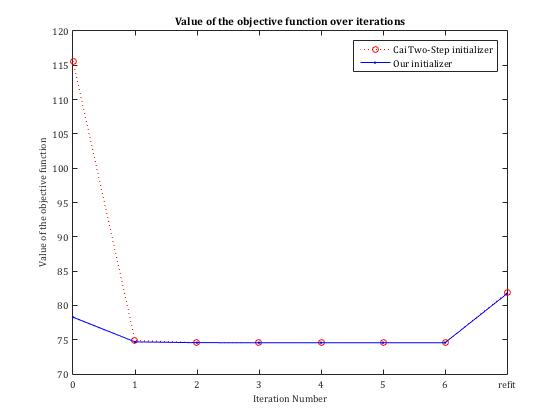
\includegraphics[scale=0.6]{Compare.jpg}
\end{figure} 
\begin{table}[h]
\centering
\caption{Change in cardinality over iterations for $B$ and $\Theta_\epsilon$} \label{tb:comparison}
\begin{tabular}{cccccccccc}
\specialrule{.1em}{0.1em}{0em} 
	& 	 & 	0 & 1 & 2 & 3 & 4 & 5 & 6 & refit \\ \hline
Our  initializer & $\widehat{B}^{(k)}$ & 275 & 275& 275& 275& 275 & 275 & 275 &  275 \\ 
	& $\widehat{\Theta}_\epsilon^{(k)}$ & 282 & 255&  247 & 247 & 248 & 248  & 248 & 260\\
CAPME initializer & $\widehat{B}^{(k)}$ &  433 & 275& 275& 275& 275 & 275 & 275 &  275 \\
					& $\widehat{\Theta}_\epsilon^{(k)}$ & 979 & 267  & 250 & 249 & 249 & 248 & 248 & 260 \\
\specialrule{.1em}{0.1em}{0em} 
\end{tabular} 
\end{table}

Based on Figure~\ref{fig:comparison} and Table~\ref{tb:comparison}, we notice that Cai et. al's two-step estimator yields larger value of the objective function compared with our initializer that is obtained through screening followed by Lasso. However, over subsequent iterations, both initializers yield the same value in the objective function, which keeps decreasing according to the nature of block-coordinate descent.  

\subsection{\normalsize Implementation issues}

Next, we introduce some acceleration techniques for the MLE algorithm aiming to reduce  computing time, yet maintaining estimation accuracy over iterations.

\medskip
\textbf{\textit{$\bs{(p_2+1)}$-block update.}} In Section \ref{sec:methodology}, we update $B$ and $\Theta_\epsilon$ by (\ref{eqn:updateB}) and (\ref{eqn:updateTheta}), respectively, and within each iteration, the updated $B$ is obtained by an application of cyclic $p_2$-block coordinate descent with respect to each of its columns until convergence. As shown in Section \ref{sec:convergence}, the outer 2-block update guarantees the MLE iterative algorithm to converge to a stationary point. However in practice, we can speed up the algorithm by updating $B$ without waiting for it to reach the minimizer for every iteration other than the first one. More precisely, for the alternating search step, we take the following steps when actually implementing the proposed algorithm with initializer $\widehat{B}^{(0)}$ and $\widehat{\Theta}_\epsilon^{(0)}$: 
\begin{itemize}
\item[--] Iteration 1: update $B$ and $\Theta_\epsilon$ as follows, respectively:
\begin{equation*}
\widehat{B}^{(1)} = \argmin\limits_{B\in \mathcal{B}_1\times \cdots\times \mathcal{B}_{p_2}} \left\{ \frac{1}{n}\sum_{i=1}^{p_2}\sum_{j=1}^{p_2}(\sigma_{\epsilon}^{ij})^{(0)}(Y_i-XB_i)^\top (Y_j - XB_j) + \lambda_n\sum_{j=1}^{p_2}\|B_j\|_1 \right\},
\end{equation*}
and
\begin{equation*}
 \widehat{\Theta}_\epsilon^{(1)} = \argmin\limits_{\Theta_\epsilon\in\mathbb{S}_{++}^{p_2\times p_2}} \left\{
 \log\det\Theta_\epsilon - \text{tr}(\widehat{S}^{(1)}\Theta_\epsilon) + \rho_n\|\Theta_\epsilon\|_{1,\text{off}}
 \right\},
 \end{equation*}
where $\widehat{S}^{(1)}$ is the sample covariance matrix of $\widehat{E}^{(1)}\equiv Y- X\widehat{B}^{(1)}$. 
\item[--] For iteration $k\geq 2$, while not converged: 
\begin{itemize}
\item[$\cdot$] For $j=1,\cdots,p_2$, update $B_j$ once by:
\begin{equation*}
\widehat{B}_j^{(k)} = \argmin\limits_{B_j\in\mathcal{B}_j} \left\{ \frac{(\sigma^{jj}_\epsilon)^{(k-1)}}{n}\|Y_j+r_j^{{(k)}}-XB_j\|_2^2 + \lambda_n\|B_j\|_1 \right\},
\end{equation*}
where 
\begin{equation}\label{eqn:updater}
r_j^{(k)} = \frac{1}{(\sigma^{jj}_\epsilon)^{(k-1)}}\left[ \sum_{i=1}^{j-1} (\sigma^{ij}_\epsilon)^{(k-1)}(Y_i-X\widehat{B}_i^{(k)}) + \sum_{i=j+1}^{p_2} (\sigma^{ij}_\epsilon)^{(k-1)} (Y_i-X\widehat{B}_i^{(k-1)})\right].
\end{equation}
\item[$\cdot$] Update $\Theta_\epsilon$ by:
\begin{equation*}
 \widehat{\Theta}_\epsilon^{(k)} = \argmin\limits_{\Theta_\epsilon\in\mathbb{S}_{++}^{p_2\times p_2}} \left\{
 \log\det\Theta_\epsilon - \text{tr}(\widehat{S}^{(k)}\Theta_\epsilon) + \rho_n\|\Theta_\epsilon\|_{1,\text{off}}
 \right\},
 \end{equation*}
 where $\widehat{S}^{(k)}$ is defined similarly. 
\end{itemize}
\end{itemize}
Intuitively, for the first iteration, we wait for the algorithm to complete the whole cyclic $p_2$ block-coordinate descent step, as the first iteration usually achieves a big improvement in the value of the objective function compared to the initialization values, as depicted in Figure~\ref{fig:comparison}.
However, in subsequent iterations, the changes in the objective function become relatively small, so we do $(p_2+1)$ successive block-updates in every iteration, and start to update $\Theta_\epsilon$ once a full $p_2$ block update in $B$ is completed, instead of waiting for the update in $B$ proceeds cyclically until convergence. In practice, this way of updating $B$ and $\Theta_\epsilon$ leads to faster convergence in terms of total computing time, yet yields the same estimates compared with the exact $2$-block update shown in Section \ref{sec:methodology}.   \\

\medskip
\textbf{\textit{Parallelization.}} A number of steps of the MLE algorithm is parallelizable. In the screening step, when applying the de-biased Lasso procedure \citep{javanmard2014confidence} to obtain the $p$-values, we need to implement $p_2$ separate regressions, which can be distributed to different compute nodes and carried out in parallel. So does the refitting step, in which we refit each column in $B$ in parallel. 

Moreover, according to \citet{bradley2011parallel,richtarik2012parallel,scherrer2012scaling} and a series of similar studies, though the block update in the alternating search step is supposed to be carried out sequentially, we can implement the update in parallel to speed up convergence, yet empirically yield identical estimates. This parallelization can be applied to either the minimization with respect to $B$ within the 2-block update method, or the minimization with respect to each column of $B$ for the $(p_2+1)$-block update method. Either way, $r_j^{(k)}$ in (\ref{eqn:updater}) is substituted by
\begin{equation*}
r_{j,\text{parallel}}^{(k)} = \frac{1}{(\sigma^{jj}_\epsilon)^{(k-1)}}\sum_{i\neq j}^{p_2} (\sigma_\epsilon^{ij})^{(k-1)}(Y_i-X\widehat{B}_i^{(k-1)}),
\end{equation*} 
which is not updated until we have updated $B_j$'s once for all $j=1,\cdots,p_2$ in parallel.\\

\medskip
The table below shows the elapsed time for carrying out our proposed algorithm using 2-block/$(p_2+1)$ -block update with/without parallelization, under the simulation setting where we have $p_1=p_2=200,n=150$. The screening step and refitting step are both carried out in parallel for all four different implementations\footnote{For parallelization, we distribute the computation on 8 cores.}. 
\begin{table}[H]
\centering
\caption{Computing time with different update methods}
\begin{tabular}{c|cccc}
\hline
	& 2-block & $(p_2+1)$-block & 2-block in parallel & $(p_2+1)$-block in parallel \\
\hline
elapsed time (sec) & 5074 & 2556 & 848 & 763 \\
\hline 
\end{tabular}
\end{table}

As shown in the table, using $(p_2+1)$-block update and parallelization both can speed up convergence and reduce computing time, which takes only 1/7 of the computing time compared with using 2-block update without parallelization.

\begin{remark}
The total computing time depends largely on the number of bootstrapped samples we choose for the stability selection step. For the above displayed results, we used 50 bootstrapped samples to obtain the weight matrix. Nevertheless, one can select the number of bootstrap samples judiciously and reduce them if performance would  not be seriously impacted.
\end{remark}











